                                                                                                                                                                                                                                                                                                                                  %% ----- PREAMBLE
\documentclass[a4paper,12pt,oneside,openany,fleqn]{uerj}

%% ----- FONTSTYLE
 %\usepackage[adobe-utopia]{mathdesign} 
\usepackage{fourier} % nicer math font style

% # Remark: Uncomment these two lines below to have Arial font in the worst case 
% 				   (UERJ's original horrible font). Owing to change of font, the footer of the title page 
%                 might leak out from the page. 
%\usepackage{helvet}
%\renewcommand{\familydefault}{\sfdefault}

%% ----- NOMENCLATURE (optional)
% Remark: the code below sorts the nomenclature in subgroups. 
%			    To have your symbols organized accordingly, use something 
% 				like the following throughout the text, provided that 'g','r','u','d','x' 
%				are kept as initial letters:
%
% 						\nomenclature[g]{$ \alpha $}{Some greek constant}
% 						\nomenclature[r]{$ t $}{Some roman variable}
% 						\nomenclature[x]{$ ( . , .) $}{Some roman variable}
%
% 				If a nomenclature section is not intended, comment all the lines. 
%
\makeindex
\makenomenclature % nomenclature
\RequirePackage{ifthen}
 \renewcommand\nomgroup[1]{%
   \ifthenelse{\equal{#1}{A}}{%
    \item[\textbf{Acronyms}] }{% A - Acronyms
     \ifthenelse{\equal{#1}{R}}{%
      \item[\textbf{Roman letters}]}{% R - Roman
       \ifthenelse{\equal{#1}{G}}{%
        \item[\textbf{Greek letters }]}{% G - Greek
         \ifthenelse{\equal{#1}{S}}{%
          \item[\textbf{Superscripts}]}{{% S - Superscripts
       \ifthenelse{\equal{#1}{U}}{%
        \item[\textbf{Subscripts }]}{{% U - Subscripts
         \ifthenelse{\equal{#1}{X}}{%
          \item[\textbf{Symbols}]}% X - Other Symbols
                    {{}}}}}}}}}} 

    
%% ----- TABLE FOOTNOTE COUNTER
\newcounter{tablenote}[table]
\newcommand{\itemx}[1]{
    \stepcounter{tablenote}
    \item[\thetablenote]\label{#1} }

%% ----- CUSTOMIZATION
\numberwithin{equation}{chapter}
\theoremstyle{plain}

% # Remark: options to redefine caption names, since Babel overwrites 
%				   definitions inside file .cls. Comment, in case of Portuguese.
%
%				   Useful options:
%								\appendixname	 Appendix
%								\bibname	 		 Bibliography (report,book)
%								\contentsname	 Contents
%								\figurename	 	 Figure (for captions)
%								\indexname	 	 Index
%								\listfigurename	 List of Figures
%								\listtablename	 List of Tables
%\pagename	 	 	 Page (letter)
%\refname	 	 	 References (article)
%\seename	 		 see (makeidx package)
%\tablename	 	 	Table (for caption)
\captionsetup[figure]{name=Figure}
\captionsetup[table]{name=Table}

%% ----- SETUP FOR REFERENCES
% 	# Remark: package 'cleveref' (pre-loaded) enables intelligent cross-referencing. 
%					however it was buggy for figure environments. 
%				    (See http://www.ctan.org/pkg/cleveref) 
%
% # Remark: the suggested use of cross-referencing is:
% 				   \cref{} for equations, sections, subsections, and chapters;
% 				   \ref{} for figures and tables;
%
% # Remark: appendices need to be written manually since the lettered 
%				   titles are not optimized for cross-reference.
%
\crefname{equation}{Equation}{Equations} % {kind}{label_singular}{label_plural}
\crefname{chapter}{Chapter}{Chapters}
\crefname{appendix}{Appendix}{Appendices}
\crefname{figure}{Figure}{Figures}
\crefname{section}{Section}{Sections}
\crefname{subsection}{Subsection}{Subsections}

%% -----  HYPERREF
% Changing standard \autoref label printing:
\renewcommand*{\tableautorefname}{Table}


%% ----- USER-DEFINED COMMANDS
% Here you may wish define your own commands
\newcommand{\Etal}{\emph{et al.}}

%% ----- HYPHENATION
% Use this command to teach words to LaTex. 
\hyphenation{en-ge-nha-ri-a}

%% ----- BEGIN OF DOCUMENT

\begin{document}

%% ----- MARKUP REFERENCES SETUPS  
% Change the values to have coloured links 
% (maybe useful for draft version or correction purposes): 
%			e.g. 'colorlinks=true', 'linkcolor=red', 'citecolor=blue', etc.
\hypersetup{    
    %colorlinks=false,    
    citecolor=black,
    filecolor=black,
    linkcolor=black,
    urlcolor=black,
    linktoc=all,   
}

%% ----- PRE-TEXTUAL ELEMENTS  (SECTION 00)
\thispagestyle{empty}\begin{titlepage}
\begin{center}

	\vspace{-0.5cm}

  \begin{figure}[hbt!]
		\begin{flushleft}
		   
\includegraphics[width=3.44cm,height=3.17cm]{logos/logo_uerj_bw}
		\end{flushleft}
	\end{figure}
	\vspace{-4cm}

  \hspace{2cm}\large{\textbf{Universidade do Estado do Rio de Janeiro}}\\
  \hspace{2cm}\large{Centro de Tecnologia e Ciências}\\
  \hspace{2cm}\large{Faculdade de Engenharia}\\

  \hspace{2cm}\large{}\\
  \hspace{2cm}\large{}\\
  \hspace{2cm}\large{}\\
  \hspace{2cm}\large{}\\

  \par
  \Large{Author's Name}

  \hspace{2cm}\large{}\\
  \hspace{2cm}\large{}\\
  \hspace{2cm}\large{}\\
  \hspace{2cm}\large{}\\


  \par
  \textbf{\LARGE Title Name }


  \par\vfill
  {\large Rio de Janeiro\\2016}

\end{center}
\end{titlepage}
\pagebreak\thispagestyle{empty}\begin{center}

{\large Author's name}

% \vfill
\vspace{2cm}

\textbf{\LARGE Title}

\vspace{1.0cm}

\begin{figure}[hbt!]
\begin{center}

\includegraphics[width=10.48cm,height=10.8cm]{logos/logo_uerj_mark}
\end{center}
\end{figure}

\vspace{-9cm}
\begin{flushright}
\parbox{8cm}{
\singlespacing{\large Tese apresentada, como requisito\linebreak parcial para obtenção do título de Doutor em Ciências, ao Programa de Pós-Graduação em Engenharia Mecânica, da Universidade do Estado do Rio de Janeiro. Área de\linebreak concentração: Fenômenos de Transporte}.
}
\end{flushright}

\vspace{4.0cm}

{\large Advisor: Prof. Ph.D. Foolan dy Tow}\\

\par\vfill
%\vspace{2cm}

{\large Rio de Janeiro\\2016}

\end{center}

\pagebreak\thispagestyle{empty}% Guideline:
% 		After finishing your paperwork, you should send a PDF of this page to the Library CTC/B at UERJ so that they check the data and 
%		approve the catalog sheet. Check the CTC/B website for updated contacts. Otherwise talk to the librarian personally. 
\begin{titlepage}
	\begin{center}
\vfill
\singlespacing
	\vspace*{85mm}
	{CATALOGAÇÃO NA FONTE\\ \vspace{1.5mm}
	UERJ\,/\,REDE SIRIUS\,/\,BIBLIOTECA CTC/B}\\
	\vspace{1.5mm}
	\begin{boxedminipage}{140mm}
	\begin{minipage}{5mm}
		\vspace{-80mm}
		O48
	\end{minipage}
	\hfill
	\raisebox{8.5mm}{
	\begin{minipage}[top]{115mm}
		\vspace*{5mm}

		Surname, Author Name.\\
		\phantom{XX}Thesis title \,/\,Author name. -- 2016.\\
		\phantom{XX}xx\,f.\\
		\phantom{XX}\\
		\phantom{XX}Orientador: Foolan dy Tow.\\
%\hspace*{5mm}
       		\phantom{XX}Tese (Doutorado) -- Universidade do Estado do Rio de Janeiro, Faculdade de Engenharia.\\
%       	\phantom{XX} Bibliografia: f.159-176.
		\phantom{XX}\\
		\phantom{XX}1.~Engenharia Mecânica. 2.~Mecânica dos fluidos -- Teses. 3.~Escoamento bifásico -- Teses. 4.~Método dos elementos finitos -- Teses. I.~Tow, Foolan dy. II.~Universidade do Estado do Rio de Janeiro. III.~Título.
	\end{minipage}}
	\vspace*{5mm}
	\begin{flushright}
	 CDU~532
	\end{flushright}
    \vspace{1mm}
	\end{boxedminipage}\\
	\end{center}
\vspace{1cm}
	Autorizo, apenas para fins acadêmicos e científicos, a reprodução total ou parcial desta dissertação, desde que citada a fonte.\\
	\noindent
	\begin{tabular}{ccc}
	\phantom{XXXXXXXXXXXXXXXXXXXXXXXXXXXXXX}&	 \phantom{XX}	&	\phantom{XXXXXXXXXXXXXXXX}	\\
	\phantom{XXXXXXXXXXXXXXXXXXXXXXXXXXXXXX}&	 \phantom{XX}	&	\phantom{XXXXXXXXXXXXXXXX}	\\
	\cline{1-1}\cline{3-3}
	Assinatura &		&	Data
	\end{tabular}
\end{titlepage}    
\pagebreak\thispagestyle{empty}\addtocounter{page}{+1}
\begin{center}

{\large Author's name}

\vspace{1cm}

\textbf{\large Title}

\end{center}

\vspace{.4cm}

\begin{flushright}
\parbox{8cm}{
\singlespacing{Tese apresentada, como requisito\linebreak parcial para obtenção do título de Doutor em Ciências, ao Programa de Pós-Graduação em Engenharia Mecânica, da Universidade do Estado do Rio de Janeiro. Área de\linebreak concentração: Fenômenos de Transporte}.
}
\end{flushright}

\vspace{.6cm}

% Date of defense; if not completed, leave it blank.
\noindent Aprovado em: 25 de dezembro de 2016

% Jury: UERJ's professors MUST BE come first, regardless whoever.
\noindent Banca Examinadora:

\vspace{.7cm}

\begin{flushright}
\parbox{12cm}{

\singlespacing

\hrulefill \\

\vspace{-.4cm}
Prof. Ph.D. Foolan dy Tow (Orientador)
\newline
Faculdade de Engenharia - UERJ
\vspace{.7cm}

\hrulefill \\

\vspace{-.4cm}
Prof. D.Sc. Cyclanus doo Mal
\newline
Instituto de Matem{\'a}tica e Estat{\'i}stica - UERJ
\vspace{.7cm}

\hrulefill \\

\vspace{-.4cm}
Prof. D.Sc. Methanus du Cow (Co-orientador)
\newline
Universidade Federal Fluminense
\vspace{.7cm}

\hrulefill \\

\vspace{-.4cm}
Prof. D.Sc. Butan of Gal
\newline
Universidade Federal do Rio de Janeiro
\vspace{.7cm}

\hrulefill \\

\vspace{-.4cm}
Prof. D.Sc. Delenis Tronxius Arymadius
\newline
Universidade Federal Fluminense
\vspace{.7cm}

}
\end{flushright}
\vfill

\begin{center}
Rio de Janeiro\linebreak 2016
\end{center}


\pagebreak\thispagestyle{empty}\begin{center}
\textbf{DEDICATION}
\end{center}

$\!$\\

%\vspace{1cm}
\null
\vfill
\begin{center}
\noindent I dedicate this thesis to my garden's lily, natural beauty, spring of my inspiration. To you, wholeheartedly. 
\end{center}




\pagebreak\thispagestyle{empty}\begin{center}
\textbf{ACKNOWLEDGMENTS}
\end{center}
$\!$\\
\par 
To Jeremiah, my father...
\par
To Elza, my mother...
\par
To Mikhailov, my cousin...
\par
To Dodonga, my puppy...
\pagebreak\thispagestyle{empty}$\!$\\

\null
\vfill
\begin{flushright}
In the midst of chaos, there is also opportunity.  \\
\vspace{0.5cm}
\textit{Sun Tzu, The Art of War}
\end{flushright}

\thispagestyle{empty}


\pagebreak\thispagestyle{empty}\begin{center}
\textbf{RESUMO}
\end{center}

% JUST ONE paragraph.
% Number of sheets (NS) = PDF pages - 2 (less cover and 2 first pages, which are printed at the same sheet)

$\!$\\

\hspace{-1.3cm}\textbf{SURNAME}, Name \textit{Title}. NS f. Tese~(Doutorado em Engenharia Mecânica) - Faculdade de Engenharia, Universidade do Estado do Rio de Janeiro~(UERJ), Rio de Janeiro, 2015.

\vspace{.2cm}

\indent \lipsum[1]

\vspace{1cm}

\hspace{-1.3cm}Palavras-chave: keyword1; keyword2; keyword3; keyword4.
\pagebreak\thispagestyle{empty}\begin{center}
\textbf{ABSTRACT}
\end{center}

% JUST ONE paragraph.
% Number of sheets (NS) = PDF pages - 2 (less cover and 2 first pages, which are printed at the same sheet)

$\!$\\

\hspace{-1.3cm}\textbf{SURNAME}, Name \textit{Title}. NS f. Tese~(Doutorado em Engenharia Mecânica) - Faculdade de Engenharia, Universidade do Estado do Rio de Janeiro~(UERJ), Rio de Janeiro, 2015.

\vspace{.2cm}

\indent \lipsum[1]

\vspace{1cm}

\hspace{-1.3cm}Keywords: keyword1; keyword2; keyword3; keyword4.

\fancypagestyle{plain}{
\fancyhf{} % clear all header and footer fields
\renewcommand{\headrulewidth}{0pt}
\renewcommand{\footrulewidth}{0pt}}
\pagestyle{plain}

\pagebreak

%% ----- LISTS  

%% LIST OF FIGURES
\def\listfigurename{LIST OF FIGURES}\listoffigures

%% LIST OF TABLES
\def\listtablename{LIST OF TABLES}\listoftables

%% LIST OF SYMBOLS {NOMENCLATURE}
\newpage
\renewcommand{\nomname}{LIST OF SYMBOLS} % redefining label
\printnomenclature % printing nomenclature in this page

%-------------------------
%% ACRONYMS
%-------------------------
%-- 3
\nomenclature[aALE]{ALE}{Arbitrary Lagrangian-Eulerian}
\nomenclature[aCVP]{CVP}{Counter-Rotating Vortex Pair}
\nomenclature[aDBC]{DBC}{Dirichlet Boundary Conditions}
\nomenclature[aDOF]{DOFs}{Degrees of Freedom}
\nomenclature[aDJICF]{DJICF}{Drop Jet in Crossflow}
\nomenclature[aFFR]{FFR}{Fixed Frame Reference}
\nomenclature[aFFT]{FFT}{Fast Fourier Transform}
\nomenclature[aPBC]{PBC}{Periodic Boundary Conditions}
\nomenclature[aVOF]{VOF}{Volume of Fluid}
%-- 2
\nomenclature[aCK]{CK}{Chemical Kinetics}
\nomenclature[aLS]{LS}{Level-Set}
\nomenclature[aRT]{RT}{Rayleigh-Taylor}
%-------------------------


%-------------------------
%% ROMAN LETTERS -- r
%-------------------------
%-- vet
\nomenclature[rcvet]{$ {\bf c} $}{relative velocity between the fluid and the mesh}
\nomenclature[rhvet]{$ {\bf h} $}{Heaviside function discrete vector}
\nomenclature[rFvet]{$ {\bf F} $}{tensor, or force}
%-- 2
\nomenclature[rA]{$ A $}{area}
\nomenclature[rB]{$ B $}{body}
\nomenclature[rF]{$ F $}{face of element}
\nomenclature[rH]{$ H $}{Heaviside function}
%--
\nomenclature[ra]{$ a $}{wave amplitude, or peak}
\nomenclature[rp]{$ p $}{hydrostatic pressure}
\nomenclature[ru]{$ u $}{arbitrary function}
\nomenclature[rf]{$ f $}{frequency}
\nomenclature[rw]{$ w $}{arbitrary weight function}
\nomenclature[rg]{$ g $ }{gravity}
\nomenclature[rbmX]{$ {\bm X} $ }{particle pathline}
\nomenclature[rbmF]{$ {\bm F} $ }{abstract source vector of fluid variables}

%-------------------------


%-------------------------
%% GREEK LETTERS -- g
%-------------------------
\nomenclature[gbmalpha]{$ {\bm \alpha} $}{backward displacement vector}
\nomenclature[gOmega]{$ \Omega $}{domain}
\nomenclature[gomega]{$ \omega $}{frequency}
\nomenclature[giota]{$ \iota $}{cardinality of nodes}
\nomenclature[gdelta]{$ \delta $}{$ \delta $ function}
\nomenclature[gdeltaz]{$ \delta_{\zeta} $}{distribution over an interface}
\nomenclature[gphi]{$ \phi $}{arbitrary scalar quantity} 
\nomenclature[gupphi]{$ \upphi $}{elongation ratio}
\nomenclature[gPsi]{$ \Psi $}{mass concentration}
\nomenclature[gpsi]{$ \psi $}{flatness ratio}
\nomenclature[gtau]{$ \tau $ }{time}
\nomenclature[grho]{$ \rho $ }{density}
\nomenclature[gvarpi]{$ \varpi $}{circulation}
%-------------------------

%-------------------------
%% SUBSCRIPTS -- u
%-------------------------
%--1
\nomenclature[u1]{$ (\cdot)_1 $}{arbitrary index, or relative to dispersed phase}
\nomenclature[u2]{$ (\cdot)_2 $}{arbitrary index, or relative to continuous phase}
\nomenclature[uA]{$ (\cdot)_A $}{relative to area}
\nomenclature[uD]{$ (\cdot)_D $}{Dirichlet}
\nomenclature[ue]{$ (\cdot)_e $}{element, or elementary}
\nomenclature[uc]{$ (\cdot)_c $}{relative to center of mass, or centroid}
%--
\nomenclature[upartial]{$ (\cdot)_\partial $}{relative to boundary}
\nomenclature[uPsi]{$ (\cdot)_\Psi$}{relative to mass concentration}
\nomenclature[urho]{$ (\cdot)_\rho $}{relative to phase}
\nomenclature[upsi]{$ (\cdot)_{\psi} $}{relative to flatness}
\nomenclature[ulambda]{$ (\cdot)_{\lambda} $}{relative to jet-to-crossflow velocity ratio}
%-- 2
\nomenclature[uNS]{$ (\cdot)_{NS} $ }{relative to Navier-Stokes}
\nomenclature[uref]{$ (\cdot)_{ref} $ }{reference}
\nomenclature[ucorr]{$ (\cdot)_{corr} $ }{correction}
\nomenclature[uhash]{$ (\cdot)_{\#} $}{provisional}
\nomenclature[urel]{$ (\cdot)_{rel} $}{relative}
\nomenclature[umov]{$ (\cdot)_{mov} $}{moving}
\nomenclature[ucrit]{$ (\cdot)_{crit} $}{critical}
%-------------------------


%-------------------------
%% SUPERSCRIPTS -- s
%-------------------------
\nomenclature[s1]{$ (\cdot)^1 $}{dispersed phase}
\nomenclature[s2]{$ (\cdot)^2 $}{continuous phase}
\nomenclature[sp]{$(\cdot)^r $}{integration order}
\nomenclature[shash]{$ (\cdot)^{\#} $}{intermediary, or provisional}
\nomenclature[ssigma]{$ (\cdot)^\sigma $}{relative to surface tension}
%-------------------------


%-------------------------
%% OTHER SYMBOLS -- x
%-------------------------
\nomenclature[xR1R2]{$ R_1, R_2 $}{principal radii of curvatures}
%-- increments
\nomenclature[xdV]{$ dV $}{infinitesimal volume}
\nomenclature[xdA]{$ dA $}{infinitesimal area}
\nomenclature[xdl]{$ dl $}{infinitesimal line}
\nomenclature[xdeltat]{$ \delta t $}{infinitesimal time}
\nomenclature[xDeltatau]{$ \Delta \tau $}{continuous time interval}
\nomenclature[xDeltat]{$ \Delta t $}{discrete time step}
\nomenclature[xpartial]{$ \partial $}{partial derivative, or boundary}
\nomenclature[xdim]{$ \dim $ }{dimension}
%--
\nomenclature[xThOmega]{$ \mathcal{T}_h^{\Omega} $}{discrete volume mesh}
\nomenclature[xThGamma]{$ \mathcal{T}_h^{\Gamma} $}{discrete surface mesh}
\nomenclature[xmathcalTh]{$ \mathcal{T}_h $}{tessellation, or triangulation, or tetrahedralization}
\nomenclature[xmathcalI]{$ \mathcal{I}_{(T)} $}{radius ratio quality measure of $ T $}
\nomenclature[xAmathcalI]{$ A_{\mathcal{I}}^{max} $}{number of tetrahedra of maximum quality }
\nomenclature[xPmathcalO]{$ \mathcal{O}_{\%} $}{mesh quality percentage at a fixed time}
%-- operators
\nomenclature[xDMaterial]{$ \dfrac{D}{Dt} $}{material derivative operator}
\nomenclature[xDMaterial]{$ \dfrac{D}{D\tau} $}{material derivative operator}
\nomenclature[xnabla]{$ \nabla $}{gradient operator}
\nomenclature[xmathsfPQ]{$ \mathsf{P},\mathsf{Q} $}{projection operators}
\nomenclature[xmathsfL]{$ \mathsf{L} $}{differential operator}
\nomenclature[xmathsfR]{$ \mathsf{R} $}{fixed reference frame}
%--
\nomenclature[xast]{$ \ast  $}{interelement Neumann contributions} 
\nomenclature[xleadsto]{$ \leadsto $}{``is associated to''}
\nomenclature[xdoteq]{$ \doteq $}{``equivalent by input argument to''}
\nomenclature[xInnerProduct]{$ (\cdot,\cdot) $ }{inner product, or bilinear form, or ordered pair}
\nomenclature[xcdot]{$ \cdot $ }{inner product}
\nomenclature[xcolon]{$ : $ }{tensor inner product}
\nomenclature[xmathring]{$ \mathring{\Omega} $}{interior of $ \Omega
 $}
\nomenclature[xvee]{$ \vee  $}{logical XOR (exclusive ``or'')}
%--
\nomenclature[xRe]{$ \Re $}{real part of a complex number} 
\nomenclature[xIm]{$ \Im $}{imaginary part of a complex number} 
\nomenclature[xotimes]{$ \otimes $}{tensor product}
\nomenclature[xoplus]{$ \oplus $}{direct sum}
\nomenclature[xdeltaip]{$ \delta_{\cdot,\cdot} $}{Kronecker's delta} 
%-- dimensionless numbers
\nomenclature[xRe]{$ Re $}{Reynolds number} 
\nomenclature[xPe]{$ Pe $}{P{\'e}clet number} 
\nomenclature[xSc]{$ Sc $}{Schmidt number} 
\nomenclature[xEu]{$ Eu $}{Euler number}
\nomenclature[xOh]{$ Oh $}{Ohnesorge number}
\nomenclature[xCa]{$ Ca $}{Capillary number}
%-- spaces
\nomenclature[xcalH1]{$ \cal{H} $}{Sobolev space }
\nomenclature[xcalL]{$ \cal{L} $}{Lebesgue space}
\nomenclature[xcalN]{$ \cal{N} $}{set of the vectors normal to a body's surface}
\nomenclature[xcalX]{$ \cal{X} $}{set of the points on a body's surface}
\nomenclature[xcalS]{$ \cal{S} $}{space of trial functions for velocity}
\nomenclature[xcalQ]{$ \cal{Q} $}{space of trial functions for pressure}








  % optional
%
% Here goes a small tutorial to compile the nomenclature file correctly. You are encouraged to look at 
% the package documentation (e.g., http://repositorios.cpai.unb.br/ctan/macros/latex/contrib/nomencl/nomencl.pdf) 
% First of all, make sure you have the package 'nomencl' installed. If so, \usepackage{nomencl} should work fine.
% Next, you should run the basic commands:
% i)  run  'pdflatex' once to generate the index files;
% ii) run the following command on terminal (or configure your IDE to do it): 
%     'makeindex thesis.nlo -s nomencl.ist -o thesis.nls'
%     ( or 'makeindex thesis.glo -s nomencl.ist -o thesis.gls', depending on your OS. Try this one if .nlo/.nls are unavailable.)
% to build the index.
% obs.: 'nomencl.ist' is the style file and it's not inside the running folder! You have to find it in your system. On Mac OS +
% Tex Live, the standard location is like: "/usr/local/texlive/2013/texmf-dist/makeindex/nomencl/nomencl.ist". Thus, the 
% previous command would be read as:
%     'makeindex thesis.nlo -s /usr/local/texlive/2013/texmf-dist/makeindex/nomencl/nomencl.ist -o thesis.nls'
% Then, 
% iii) run 'pdflatex' again.
% Afterwards, you should have the nomenclature compiled if all is OK. In case of problems, verify if you are calling the commands
% to settle the nomenclature correctly; if you are appending the 'input' directives for the files where the nomenclatures are included;
% if after calling 'makeindex', it outputs information about nomenclature entries found. 
% That's all (about tex)! 


%% ----------------------------------------------
%%				   CONTENTS  
%% ----------------------------------------------
\def\contentsname{CONTENTS}\tableofcontents

%% ----------------------------------------------
%%				   CUSTOMISATION  
%% ----------------------------------------------
\fancypagestyle{plain}{
\fancyhf{} % clear all header and footer fields
\fancyhead[R]{\thepage}
\setlength{\voffset}{-1cm}
\setlength{\headsep}{1cm}
\renewcommand{\headrulewidth}{0pt}
\renewcommand{\footrulewidth}{0pt}}
\pagestyle{plain}

\pagebreak
%% -----  PEER-REVIEW STYLE  
%\linenumbers % numbering lines here. Uncomment in the final version. 
%\doublespacing % double spacing from here. Uncomment in the final version.

%% ----- INTRODUCTION  (01)
\addcontentsline{toc}{chapter}{\hspace{1.7cm}\bfseries INTRODUCTION}
\noindent\textbf{INTRODUCTION}
\\

Happiness is difficult to be defined. However, it can be inferred by experience that the mankind seeks for a welfare which is ruled by this word. Since long time ago, many people living on Earth have been brooding over an ideal way to have good days. In this thesis, some features that lead to happiness are investigated with basis on the experience of Logophorus of Klektos while he had wandered on the edge between the pleasurable and the squalid lifestyle. 



%% ----- CHAPTERS  (02)
\chapter{\textbf{CHAPTER NAME}}
\label{chap:chapname}

\lipsum[1]

\section{\textbf{Section name format}} 
\label{sec:secname}

\lipsum[2-3]
\begin{figure}
\centering	
		\centering
		\subfloat[]{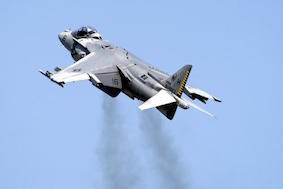
\includegraphics[scale=0.7]{figs/chap1/fig1.jpg} }
		\hspace{0.2cm}
		\subfloat[]{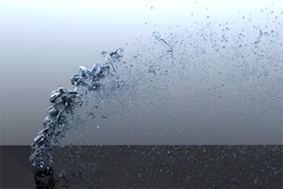
\includegraphics[scale=0.7]{figs/chap1/fig2.jpg} } \\
		\bigskip
\caption[Images from internet sites exemplifying physical conditions in which JICF configurations are detected]{\label{fig:jicf-examples}Images from internet sites exemplifying physical conditions in which JICF configurations are detected: (a) an AV-8B Harrier aircraft during vertical taking-off process; (b) atomization of an aircraft engine liquid fuel jet in a crossflow.}
\end{figure}

\lipsum[1-4]

\section{\textbf{Section name}}

Under the motivational aspects previously reviewed, this thesis:
\begin{itemize}
\item do A
\item do B and
\item do C
\end{itemize}


\section{\textbf{Citations}}

Special contents about JICF are found in Karagozian, Cortelezzi and Soldati \cite{KaragozianBook2003} and Mahesh \cite{Mahesh2013}. 

\chapter{\textbf{CHAPTER NAME 2}} 

\section{\textbf{Section name}}

\subsection{\underline{Subsection name}}

\lipsum[1-2]
\begin{subequations}
\begin{align} 
v_r(t) &= 0 \label{eq:taylor-v1} \\
v_{\theta}(t) &= \varpi r \exp \left( - \dfrac{r^2}{4r_cRe^{-1}}t \right)  \label{eq:taylor-v2} \\
v_z(t) &= 0 \label{eq:taylor-v3}
\end{align}
\end{subequations}

\lipsum[2-5]

\begin{table}
\centering
\begin{tabular}{ll}
\toprule
Parameter & Value \\
\midrule
$ r_c $          		  & $ L_{ref}/30 $ \\ 
$ U_{ref} $            & $ 1 $	              \\
$ \varpi $              & $ 1 $				  \\
$ Re $                    & $ 35 $  			  \\
$ Sc $                    & $ 650 $  		   \\
$ \Delta t $           & $ 0.1 $              \\
\bottomrule
\end{tabular}
\caption{Physical parameters of the Taylor vortex flow.}
\label{tbl:taylor-vortex-parameters}
\end{table}

\section{\textbf{Equations}}

\lipsum[1-3]
\begin{equation}
\label{eq:Eu}
Eu_{\beta} = \frac{\beta_0}{\rho^2 g_{ref}},  \lambda = \frac{L_P}{D_b}.
\end{equation}



%% ----- CONCLUSION  (03)
\pagebreak
\addcontentsline{toc}{chapter}{\hspace{1.7cm}\bfseries CONCLUSION}
\clearpage
\noindent\textbf{CONCLUSION}
$\!$\\

\lipsum[3-5]

Some directions for future work are the following:
\begin{itemize}
\item A
\item B
\item C
\end{itemize}

To conclude, be happy because you will get on there!











%% ----- APPENDICES  (04) - optional
\pagebreak
\addcontentsline{toc}{chapter}{\hspace{1.7cm}\bfseries APPENDIX A - VITA}
\noindent{\textbf{APPENDIX A - VITA}
\bigskip

\lipsum[1]



%% ----- REFERENCES  
\pagebreak
\addcontentsline{toc}{chapter}{\hspace{1.7cm}\bfseries REFERENCES}
\def\bibname{REFERENCES}

%% ----- BIBTEX DATABASE
\bibliographystyle{abnt-num}
\bibliography{refs}	 % bibtex entries or 
%\bibliography{../../bib}	 % full path to bib database
\end{document}

%% -----END OF DOCUMENT

